\documentclass[landscape]{article}

\usepackage[utf8]{inputenc}
\usepackage[english]{babel}

\usepackage{amsmath,amsfonts,amssymb}
\usepackage{fullpage}
\usepackage{verbatim}

\usepackage{tikz}
\usetikzlibrary{patterns}

% ------------------------------------------------------------------------------
% PgfPlots with TikZ

\usepackage{pgfplots}
\pgfplotsset{compat=1.12}

\usepgfplotslibrary{groupplots}

% space instead of thousand separator comma
\pgfkeys{/pgf/number format/.cd,1000 sep={\,}}

% another ylabel on the right:
\pgfplotsset{
    ylabel right/.style={
        after end axis/.append code={
            \node [rotate=270, anchor=south, yshift=3pt] at (rel axis cs:1,0.5) {#1};
        }
    }
}

\pgfplotsset{
    log x ticks with fixed point/.style={
        xticklabel={
            \pgfkeys{/pgf/fpu=true}
            \pgfmathparse{exp(\tick)}%
            \pgfmathprintnumber[fixed relative, precision=3]{\pgfmathresult}
            \pgfkeys{/pgf/fpu=false}
        }
    },
    log y ticks with fixed point/.style={
        yticklabel={
            \pgfkeys{/pgf/fpu=true}
            \pgfmathparse{exp(\tick)}%
            \pgfmathprintnumber[fixed relative, precision=3]{\pgfmathresult}
            \pgfkeys{/pgf/fpu=false}
        }
    }
}

\pgfplotsset{
    grid,
    major grid style={thin,dotted,color=black!50},
    minor grid style={thin,dotted,color=black!50},
    legend cell align=left,
    cycle list name={exotic},
    every axis/.append style={
        line width=0.5pt,
        tick style={
            line cap=round,
            thin,
            major tick length=4pt,
            minor tick length=2pt,
        },
    },
    legend style={
        /tikz/every even column/.append style={column sep=3mm,black},
        /tikz/every odd column/.append style={black},
    },
    % move title closer
    title style={yshift=-2pt},
    % less space on left and right
    enlarge x limits=0.04,
    every tick label/.append style={font=\small},
    %every axis label/.append style={font=\small},
    every axis y label/.append style={yshift=-1ex},
    xlabel near ticks,
    ylabel near ticks,
    legend columns=1,
    legend pos=north east,
}

\pgfplotsset{
    landscapePlot/.style={
        ybar,
        xtick=data,
        width=110mm,height=105mm,
        nodes near coords,
        nodes near coords align={vertical},
        enlarge y limits={upper,value=0.2},
        ymin=0,
        enlarge x limits=0.5,
    },
    batchTimePlot/.style={
        landscapePlot,
        title={Runtime},
        ylabel={SA construction time [s]},
        every axis y label/.style={at={(0,0.5)},xshift=-25pt,rotate=90},
    },
    batchMemPlot/.style={
        landscapePlot,
        title={Memory Utilization},
        ylabel={Extra Memory [MB]},
        every axis y label/.style={at={(0,0.5)},xshift=-34pt,rotate=90},
    },
}

%%%%%%%%%%%%%%%%%%%%%%%%%%%%%%%%%%%%%%%%%%%%%%%%%%%%%%%%%%%%%%%%%%%%%%%%%%%%%%%%

\begin{document}

\pgfplotscreateplotcyclelist{exotic}{%
    {fill=teal!50!white},
    {fill=orange!80!white},
    {fill=cyan!80!white},
    {fill=lime!80!white},
    {fill=red!80!white},
    {fill=yellow!80!white},
    {fill=black!60!white},
    {fill=blue!80!white},
    {fill=teal!80!white, postaction={pattern=north east lines}},
    {fill=orange!80!white, postaction={pattern=north east lines}},
    {fill=cyan!80!white, postaction={pattern=north east lines}},
    {fill=lime!80!white, postaction={pattern=north east lines}},
    {fill=red!80!white, postaction={pattern=north east lines}},
    {fill=yellow!80!white, postaction={pattern=north east lines}},
    {fill=black!30!white, postaction={pattern=north east lines}},
    {fill=blue!80!white, postaction={pattern=north east lines}},
    {fill=teal!80!white, postaction={pattern=north west lines}},
    {fill=orange!80!white, postaction={pattern=north west lines}},
    {fill=cyan!80!white, postaction={pattern=north west lines}},
    {fill=lime!80!white, postaction={pattern=north west lines}},
    {fill=red!80!white, postaction={pattern=north west lines}},
    {fill=yellow!80!white, postaction={pattern=north west lines}},
    {fill=black!30!white, postaction={pattern=north west lines}},
    {fill=blue!80!white, postaction={pattern=north west lines}},
    {fill=teal!80!white, postaction={pattern=horizontal lines}},
    {fill=orange!80!white, postaction={pattern=horizontal lines}},
    {fill=cyan!80!white, postaction={pattern=horizontal lines}},
    {fill=lime!80!white, postaction={pattern=horizontal lines}},
    {fill=red!80!white, postaction={pattern=horizontal lines}},
    {fill=yellow!80!white, postaction={pattern=horizontal lines}},
    {fill=black!30!white, postaction={pattern=horizontal lines}},
    {fill=blue!80!white, postaction={pattern=horizontal lines}},
    {fill=teal!80!white, postaction={pattern=crosshatch}},
    {fill=orange!80!white, postaction={pattern=crosshatch}},
    {fill=cyan!80!white, postaction={pattern=crosshatch}},
    {fill=lime!80!white, postaction={pattern=crosshatch}},
    {fill=red!80!white, postaction={pattern=crosshatch}},
    {fill=yellow!80!white, postaction={pattern=crosshatch}},
    {fill=black!30!white, postaction={pattern=crosshatch}},
    {fill=blue!80!white, postaction={pattern=crosshatch}},
    {fill=teal!80!white, postaction={pattern=crosshatch dots}},
    {fill=orange!80!white, postaction={pattern=crosshatch dots}},
    {fill=cyan!80!white, postaction={pattern=crosshatch dots}},
    {fill=lime!80!white, postaction={pattern=crosshatch dots}},
    {fill=red!80!white, postaction={pattern=crosshatch dots}},
    {fill=yellow!80!white, postaction={pattern=crosshatch dots}},
    {fill=black!30!white, postaction={pattern=crosshatch dots}},
    {fill=blue!80!white, postaction={pattern=crosshatch dots}},
    {fill=teal!80!white, postaction={pattern=fivepointed stars}},
    {fill=orange!80!white, postaction={pattern=fivepointed stars}},
    {fill=cyan!80!white, postaction={pattern=fivepointed stars}},
    {fill=lime!80!white, postaction={pattern=fivepointed stars}},
    {fill=red!80!white, postaction={pattern=fivepointed stars}},
    {fill=yellow!80!white, postaction={pattern=fivepointed stars}},
    {fill=black!30!white, postaction={pattern=fivepointed stars}},
    {fill=blue!80!white, postaction={pattern=fivepointed stars}},
    }

% IMPORT-DATA phases result/result_phases.txt

\begin{figure}
    \centering\small

    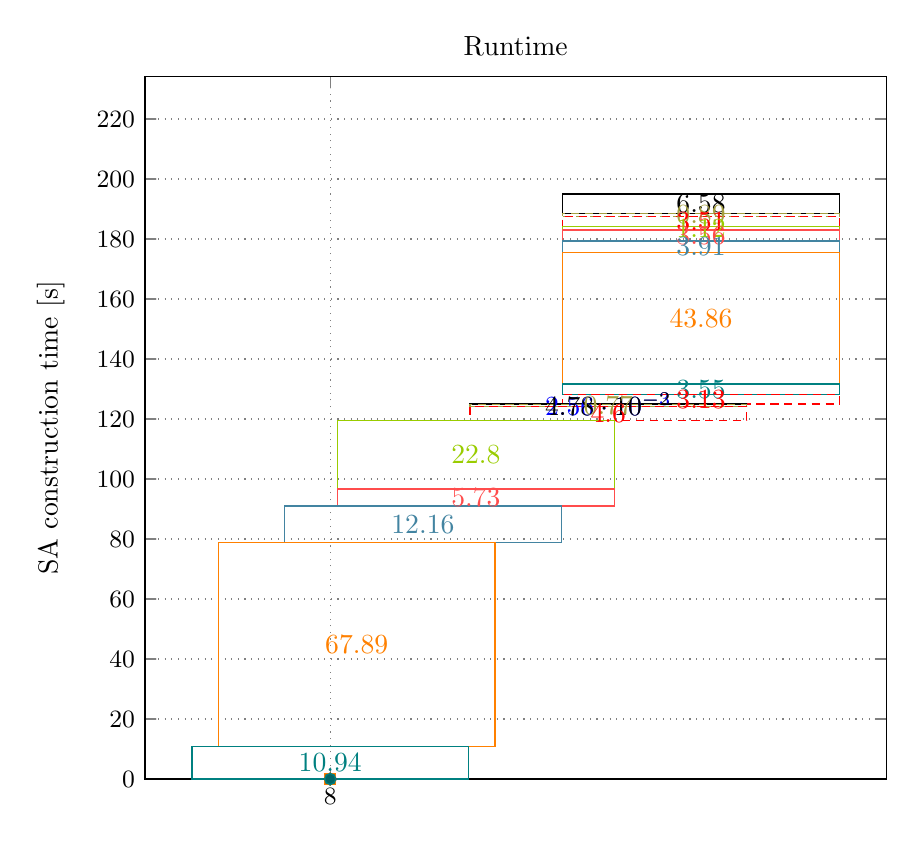
\begin{tikzpicture}
        \begin{axis}[
                ybar stacked,
                bar width=100pt,
                xtick=data,
                width=110mm,height=105mm,
                nodes near coords,
                enlarge y limits={upper,value=0.2},
                ymin=0,
                enlarge x limits=0.5,
                title={Runtime},
                ylabel={SA construction time [s]},
                every axis y label/.style={at={(0,0.5)},xshift=-34pt,rotate=90},
                cycle list name={exotic},
                legend to name=legend0,
                legend style={
                    /tikz/every even column/.append style={column sep=0.5cm,black},
                    /tikz/every even column/.append style={black},
                },
                legend columns=4,
                %symbolic x coords={pc\_dna.200MB},
                %every node near coord/.append style={color=black, rotate=90, anchor=west},
            ]

            %% MULTIPLOT(phase_name) SELECT phase_name, id AS x, time AS y
            %% FROM (
            %%      SELECT id, phase_id, phase_name, MEDIAN(memPeak) AS memPeak, MEDIAN(time) AS time FROM phases GROUP BY phase_id
            %% ) GROUP BY MULTIPLOT,x ORDER BY phase_id
            \addplot coordinates { (8,10.9363) };
            \addlegendentry{phase\_name=Main Phase};
            \addplot coordinates { (10,67.891) };
            \addlegendentry{phase\_name=Reference implementation};
            \addplot coordinates { (15,12.1595) };
            \addlegendentry{phase\_name=Phase 3};
            \addplot coordinates { (19,5.72991) };
            \addlegendentry{phase\_name=Iteration};
            \addplot coordinates { (19,22.8043) };
            \addlegendentry{phase\_name=Write out result};
            \addplot coordinates { (29,4.60052) };
            \addlegendentry{phase\_name=Update(h=32)};
            \addplot coordinates { (29,0.76913) };
            \addlegendentry{phase\_name=Update(h=64)};
            \addplot coordinates { (29,0.0478305) };
            \addlegendentry{phase\_name=Update(h=128)};
            \addplot coordinates { (29,0.002555) };
            \addlegendentry{phase\_name=ISA to SA};
            \addplot coordinates { (36,3.13236) };
            \addlegendentry{phase\_name=Copy SA\_0 and SA\_12 into l-type-positions of out\_sa};
            \addplot coordinates { (36,3.54757) };
            \addlegendentry{phase\_name=Calculate ISA\_0 and ISA\_12 into s-type-positions of out\_sa};
            \addplot coordinates { (36,43.8602) };
            \addlegendentry{phase\_name=Merge SA\_0 and SA\_12};
            \addplot coordinates { (36,3.91031) };
            \addlegendentry{phase\_name=Update ISA\_0 and ISA\_12 with positions in merged arrays};
            \addplot coordinates { (36,3.56057) };
            \addlegendentry{phase\_name=Move ISA\_012 to the end of out\_sa};
            \addplot coordinates { (36,1.11727) };
            \addlegendentry{phase\_name=Calculate SA\_012};
            \addplot coordinates { (36,3.51053) };
            \addlegendentry{phase\_name=Calculate position array of s-type-positions};
            \addplot coordinates { (36,0.891713) };
            \addlegendentry{phase\_name=Update SA\_012 with s-type-positions};
            \addplot coordinates { (36,6.58248) };
            \addlegendentry{phase\_name=Induce SA};
        \end{axis}
    \end{tikzpicture}
    \hfill
    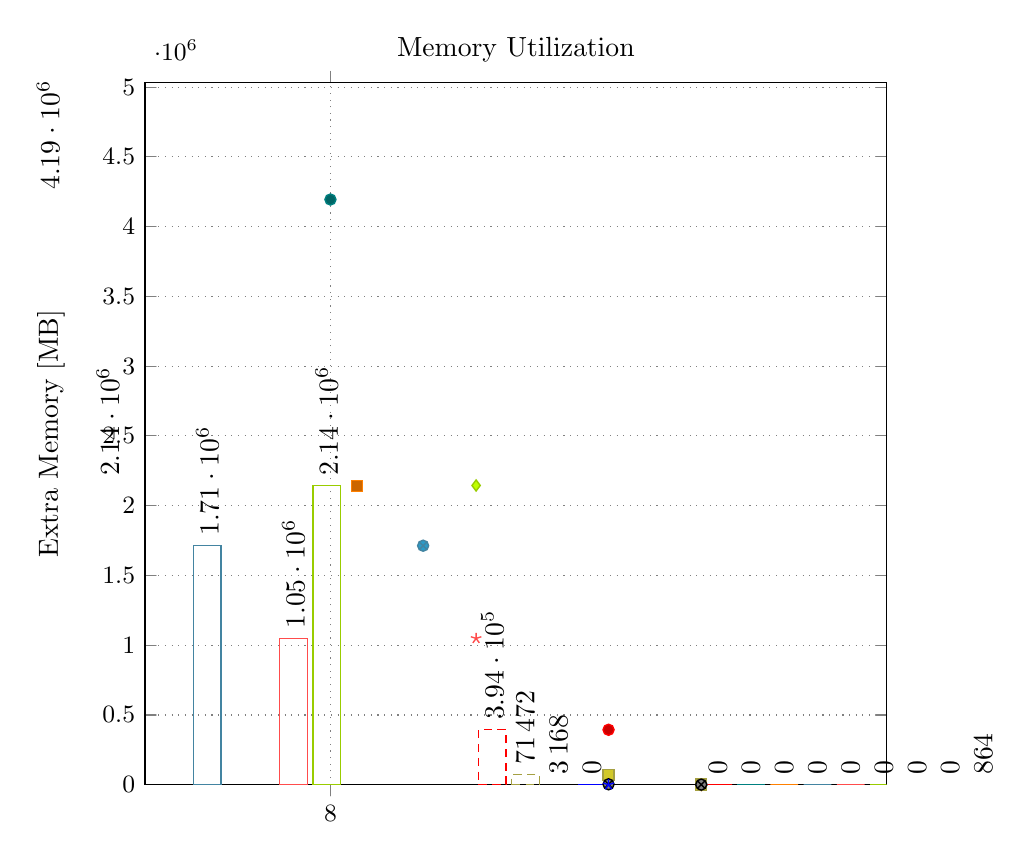
\begin{tikzpicture}
        \begin{axis}[batchMemPlot,
                cycle list name={exotic},
                legend to name=legend0,
                legend style={
                    /tikz/every even column/.append style={column sep=0.5cm,black},
                    /tikz/every even column/.append style={black},
                },
                legend columns=4,
                %symbolic x coords={pc\_dna.200MB},
                every node near coord/.append style={color=black, rotate=90, anchor=west},
            ]

            %% MULTIPLOT(phase_name) SELECT phase_name, id AS x, memPeak AS y
            %% FROM (
            %%      SELECT id, phase_id, phase_name, MEDIAN(memPeak) AS memPeak, MEDIAN(time) AS time FROM phases GROUP BY phase_id
            %% ) GROUP BY MULTIPLOT,x ORDER BY phase_id
            \addplot coordinates { (8,4194308) };
            \addlegendentry{phase\_name=Main Phase};
            \addplot coordinates { (10,2142304) };
            \addlegendentry{phase\_name=Reference implementation};
            \addplot coordinates { (15,1.71306e+06) };
            \addlegendentry{phase\_name=Phase 3};
            \addplot coordinates { (19,1048577) };
            \addlegendentry{phase\_name=Iteration};
            \addplot coordinates { (19,2144832) };
            \addlegendentry{phase\_name=Write out result};
            \addplot coordinates { (29,393852) };
            \addlegendentry{phase\_name=Update(h=32)};
            \addplot coordinates { (29,71472) };
            \addlegendentry{phase\_name=Update(h=64)};
            \addplot coordinates { (29,3168) };
            \addlegendentry{phase\_name=Update(h=128)};
            \addplot coordinates { (29,0) };
            \addlegendentry{phase\_name=ISA to SA};
            \addplot coordinates { (36,0) };
            \addlegendentry{phase\_name=Copy SA\_0 and SA\_12 into l-type-positions of out\_sa};
            \addplot coordinates { (36,0) };
            \addlegendentry{phase\_name=Calculate ISA\_0 and ISA\_12 into s-type-positions of out\_sa};
            \addplot coordinates { (36,0) };
            \addlegendentry{phase\_name=Merge SA\_0 and SA\_12};
            \addplot coordinates { (36,0) };
            \addlegendentry{phase\_name=Update ISA\_0 and ISA\_12 with positions in merged arrays};
            \addplot coordinates { (36,0) };
            \addlegendentry{phase\_name=Move ISA\_012 to the end of out\_sa};
            \addplot coordinates { (36,0) };
            \addlegendentry{phase\_name=Calculate SA\_012};
            \addplot coordinates { (36,0) };
            \addlegendentry{phase\_name=Calculate position array of s-type-positions};
            \addplot coordinates { (36,0) };
            \addlegendentry{phase\_name=Update SA\_012 with s-type-positions};
            \addplot coordinates { (36,864) };
            \addlegendentry{phase\_name=Induce SA};
        \end{axis}
    \end{tikzpicture}
    \medskip
    \ref{legend0}
\end{figure}

\end{document}

